\chapter{CheCoPro}\label{CH}

独立同期モデルに基づいて,協調プログラミング支援システムCheCoPro(Cheerful Collaborative Programming)を設計・実装した.CheCoProはクライアント・サーバ方式を利用したシステムである.サーバは新規開発し,クライアントは,我々が開発し,授業で利用しているプログラミング初学者用の開発環境上に組み込む形で実装した.開発言語はクライアント・サーバともにJava(version 1.8)である.

%----------5.1--------
\section{インタフェース}

\begin{figure}[tb]
	\begin{center}
		\includegraphics[width=\linewidth]{img/Interface.eps}
		\caption{CheCoProによるファイル共有の概略図}
		\label{fig:ev}
	\end{center}
\end{figure}


\begin{figure}[tb]
	\begin{center}
		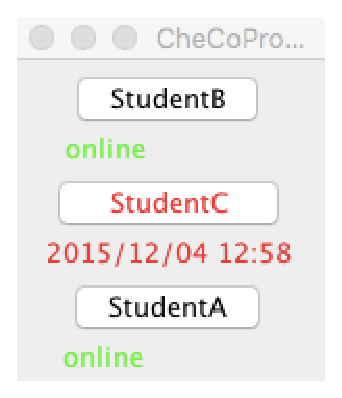
\includegraphics[scale = 0.5]{img/member.eps}
		\caption{メンバセレクタ}
		\label{fig:ms}
	\end{center}
\end{figure}

\begin{figure}[tb]
	\begin{center}
		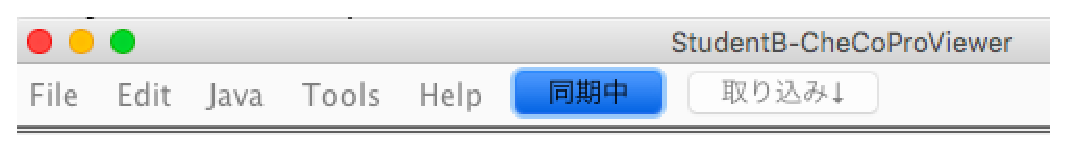
\includegraphics[width=\linewidth]{img/menu.eps}
		\caption{メニューバー}
		\label{fig:mb}
	\end{center}
\end{figure}

CheCoProによるファイル共有の概略図を\figref{fig:ev}に示す.エディタは自身のプログラムを記述するためのウィンドウである.ビューアはメンバのプロジェクトを閲覧するためのウィンドウである.ビューアは,メンバセレクタ(\figref{fig:ms})上のメンバのIDが表示されたボタンをクリックすることで開く.メンバセレクタ上に黒字で表示されているメンバはオンラインであり,赤字で表示されているメンバはオフラインである.ビューアのメニューバー(\figref{fig:mb})から同期状態にするか否かや,全部取込操作を行うことができる.

以下,同期機能と取り込み機能の詳細を説明する.


%----------5.2--------
\section{同期機能}

同期機能は,グループメンバの最新のプロジェクトをリアルタイムに受け取り,それを観察できる機能である.ユーザが自身のエディタ上でソースコードの編集を行うと,その様子が他のメンバのビューアにリアルタイムに反映される.ビューアでは,編集を観察するだけでなく,プログラムを実行して動作を確認することも可能である.

ビューアではソースコードの編集ができない.つまり,他のメンバのソースコードを直接変更できない仕様である.これは独立同期モデルに基づいた設計である.他のメンバのソースコードを編集したい場合,編集したいソースコードを取り込み自分の変更を加え,他のメンバが取り込むという手順が必要である.

ビューアのメニューバーから同期/非同期の切り替えを可能とした理由は,ビューアからメンバのプログラムを実行可能にするためである.同期中はメンバの変更をリアルタイムに受け取るため,プログラムをコンパイルし,実行することができない.非同期中に切り替え,コンパイルエラーが発生するような状態なら自身で修正をして実行することができる.


%----------5.3--------
\section{取り込み機能}

取り込み機能とは,単純な操作でグループメンバのファイルを取り込むことができる機能である.CheCoProでは,2種類の単純な取り込み方法を提供している.1つは全部取込であり,もう1つは部分取込である.

全部取込は,1人のグループメンバが持っているファイルを1度に全て取り込むというものである.全部取込を行う際に,プロジェクトの中のファイルを全て取り込むか,ソースファイル(Javaファイル)を取り込むか,素材ファイル(画像や音楽ファイル)を取り込むかを選択することが可能である.取り込む際に,自身のプロジェクトに同名ファイルが存在する場合は上書きされる.

部分取込は,コピー\&ペーストによる手動の取り込み方法である.ユーザはビューアから取り込みたい部分をコピーし,エディタ上に貼り付けるという単純操作でソースコードを取り込むことができる.

以上の2点の操作には特別な知識は必要としないため,初心者でも容易に行うことができると考えられる.